\section{Correlation between Submission Properties and Detection Rate}
\label{sec:corr}
This section presents our study of the correlation between various properties of \pe\ submissions and the detection rate of \pe\ submissions.
Detection rate is what most \vt\ users use to decide whether their submissions are benign or malware 
and the first thing that a user of \vt\ uses.
Therefore, it is important to study what factors affects or correlates to detection rate
and the results can guide security researchers and vendors to invest \yiying{TODO}. 

We studied a range of properties and their correlation with detection rate
and found that three factors have higher correlation:
submission file size,
historical submission properties, and the reputation of source IDs.
We present these correlation study results in this section.
In the next section, we will present our further analysis of what can affect the detection result of anti-virus engines
and if detection rate is a perfect measurement of the likelihood of malware.
%Detection rate is a good indication of the likelihood of malware.
%A higher detection rate means that more anti-virus engines identify a submitted file as malicious.
%\yiying{Can we say that higher detection rate indicates that the file is likely to be a malware?}
%Our study is conducted from four aspects: reputation of source id, submission history, 
%file size, and source country.

%\begin{figure*}[!htb]
\minipage{0.31\textwidth}
  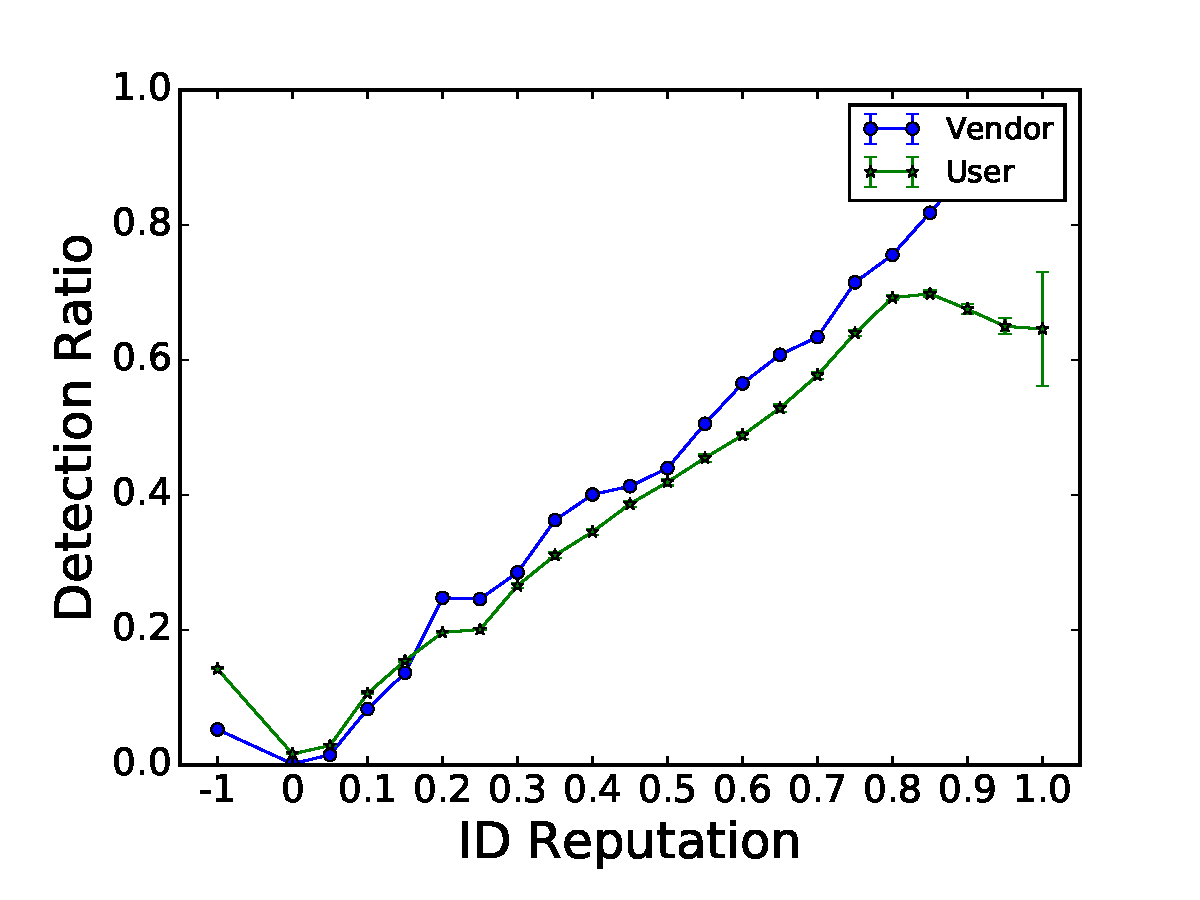
\includegraphics[width=\linewidth]{figure/IDReputation}
  \mycaption{fig:idreputation}{The relation between source id's previous reputation and detection rate.}
{\footnotesize{(How detection rate changes with the value of source id's reputation. Each reputation is rounded up to nearest 0.05.
Reputation -1 means the source id did not make any submission before. 95\% confidence interval is also drawn 
for each point.)}}
\endminipage\hfill
\minipage{0.31\textwidth}
  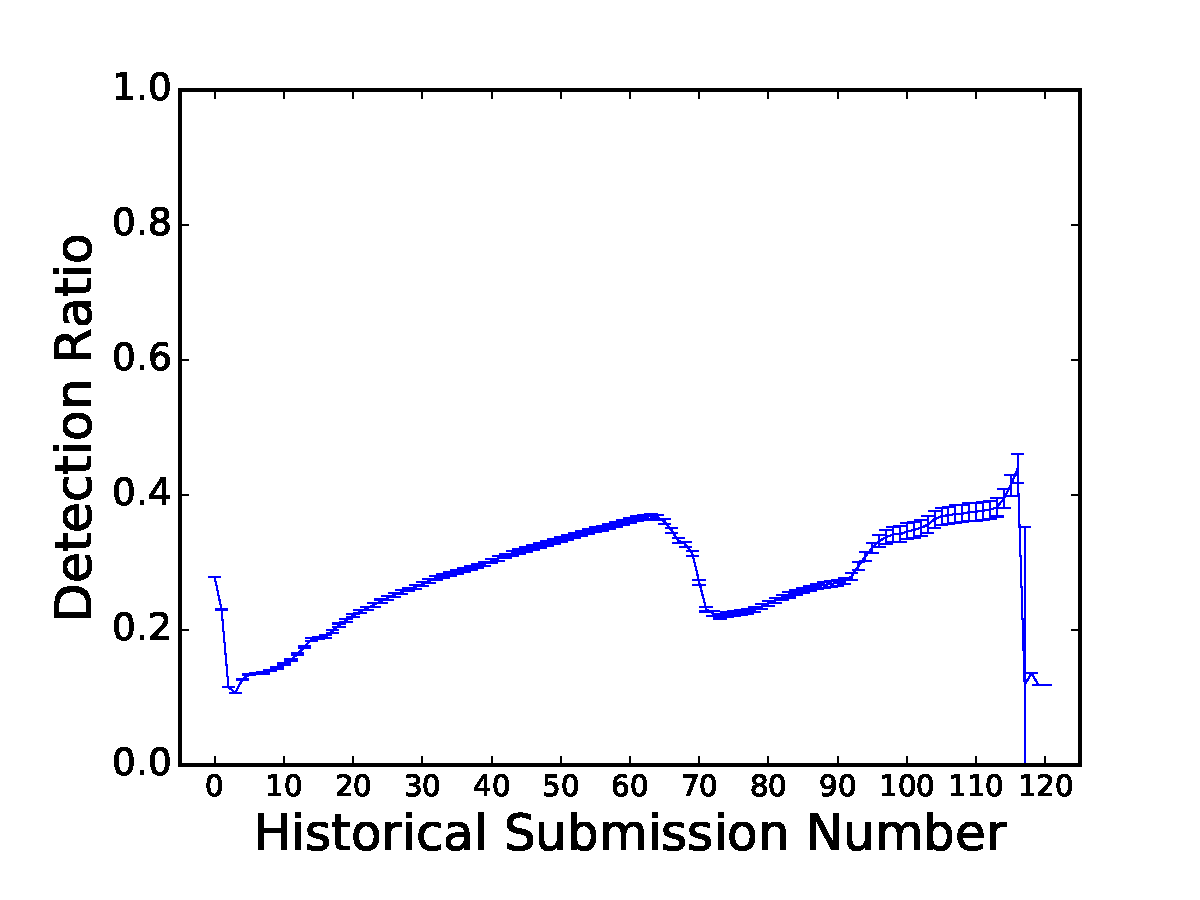
\includegraphics[width=\linewidth]{figure/SubNum}
  \mycaption{fig:hisnum}{The relation between historical submission number and detection rate.}
  {\footnotesize{(How detection rate changes with historical submission number. 
Each historical number is rounded up to nearest 5.
95\% confidence interval is also drawn for each point.)}}
\endminipage\hfill
\minipage{0.31\textwidth}%
  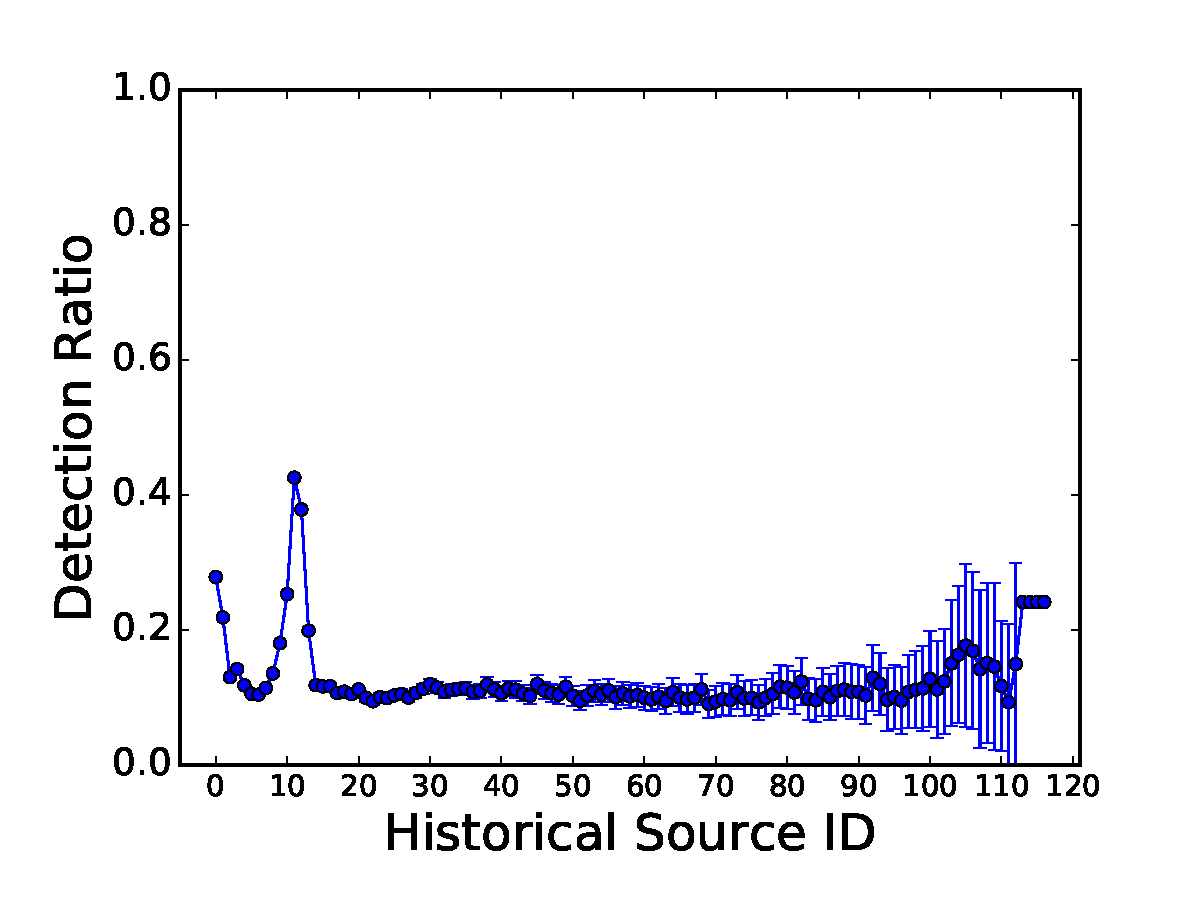
\includegraphics[width=\linewidth]{figure/SubID}
  \mycaption{fig:hisid}{The relation between the number of historical source ids and detection rate.}
{\footnotesize{(How detection rate changes with the number of historical source ids. 
Each historical number of source ids is rounded up to nearest 5.
95\% confidence interval is also drawn for each point.)}}
\endminipage\hfill

%\vspace{-0.2in}
\end{figure*}


\begin{figure}[t!]
\begin{center}
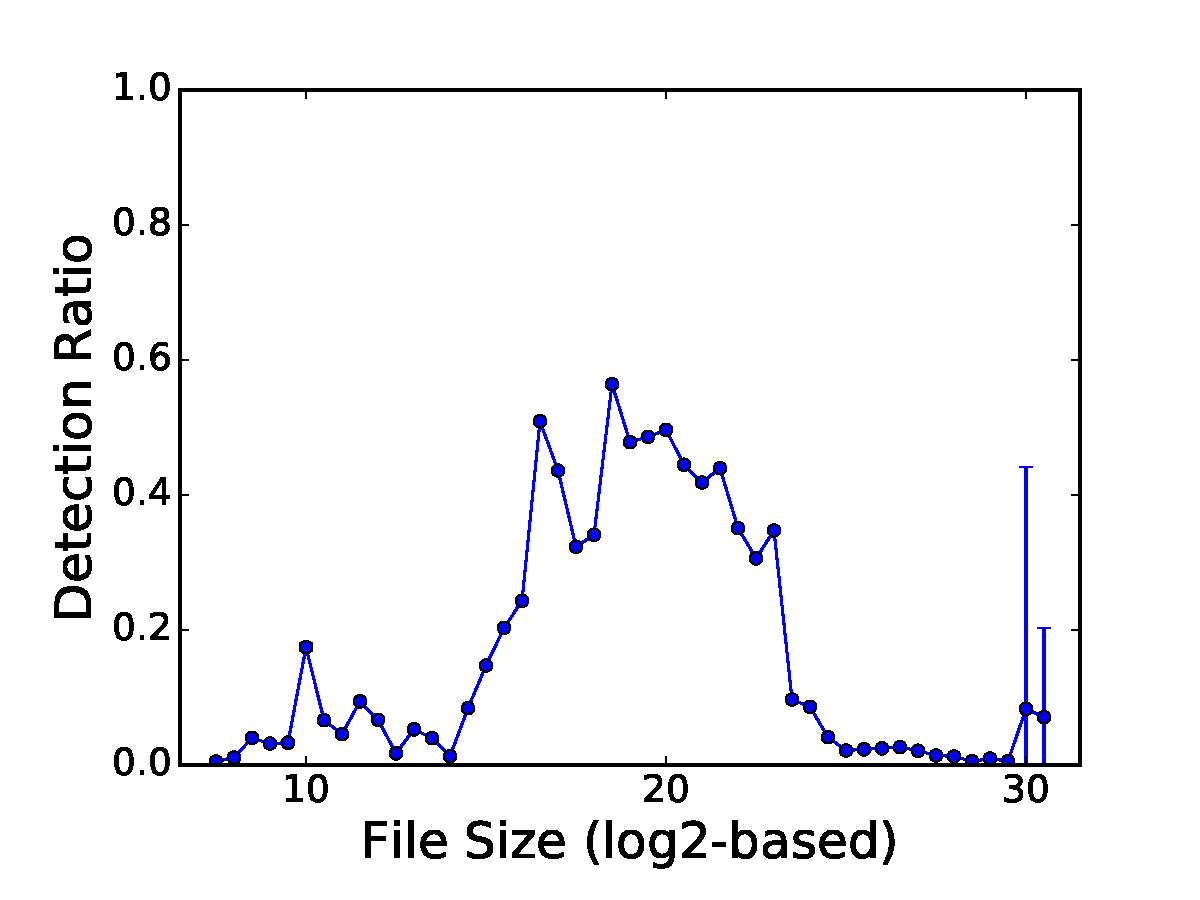
\includegraphics[width=2in]{figure/size}
  \caption{How detection rate changes with file size.
(
95\% confidence interval is also drawn for each point.
Results of log2 for the original file sizes are rounded to the nearest 0.5 value.)
}
\label{fig:size}
\end{center}
%\vspace{-0.25in}
\end{figure}


\subsection{File Size}
\label{sec:size}
Anecdotely, \pe\ malwares are most likely to have small to medium size. 
To verify this, we analyzed the relationship between submission file size and detection rate. 
Figure~\ref{fig:size} presents the average detection rate and 
the 95\% confidence interval for different file sizes.
A wider confidence interval implies that \yiying{fill here}.
We use discrete file sizes of powers of two in our analysis and in this graph,
i.e., we calculate the log2 of each original file size and round it to the nearest 0.5 value.
Overall, we find that files with size from 90KB to 4MB have higher detection rate, more than 20\% on average. 
Except for the last two points which represent a small amount of files that are bigger than 1GB, 
all other sizes have high confidence.   

{\bf Observation 4:} 
{\em \pe\ malwares are mostly likely to have small to medium size.}

An immediate question to raise is whether the high detection rate of files with small to medium size
is because these files also contribute to most of the submissions as shown in Figure~\ref{fig:pesize}.
As we will discuss in Section~\ref{sec:history}, the correlation of submissions and detection rate is more complex and non-linear.
Thus, there is a more fundamental reason behind the file size correlation with detection rate.
One likely reason of this correlation is that files that are too small are not enough to express the
malware functions while files that are too big is \yiying{fill here}.

\if 0
\subsection{Source Country}
\label{sec:country}

All PE submissions in our collection are conducted from 222 countries, 
and for roughly 17\% PE submissions, 
VirusTotal fails to provide their source country information. 
We rank source countries, based on their submission numbers. 
Average detection rate for top 20 source countries are calculated and shown in 
Figure~\ref{fig:Country}. 
Confidence intervals are also drawn for each source country, 
and all confidence intervals are almost invisible. 
From Figure~\ref{fig:Country}, 
we can see that submissions source countries are correlated with detection rate.
\yiying{What's the order of the x axis in this figure? we should either sort it alphabetically or by detection rate.}

\fi


\subsection{Submission History}
\label{sec:history}

%\begin{figure*}[!htb]
\minipage{0.31\textwidth}
  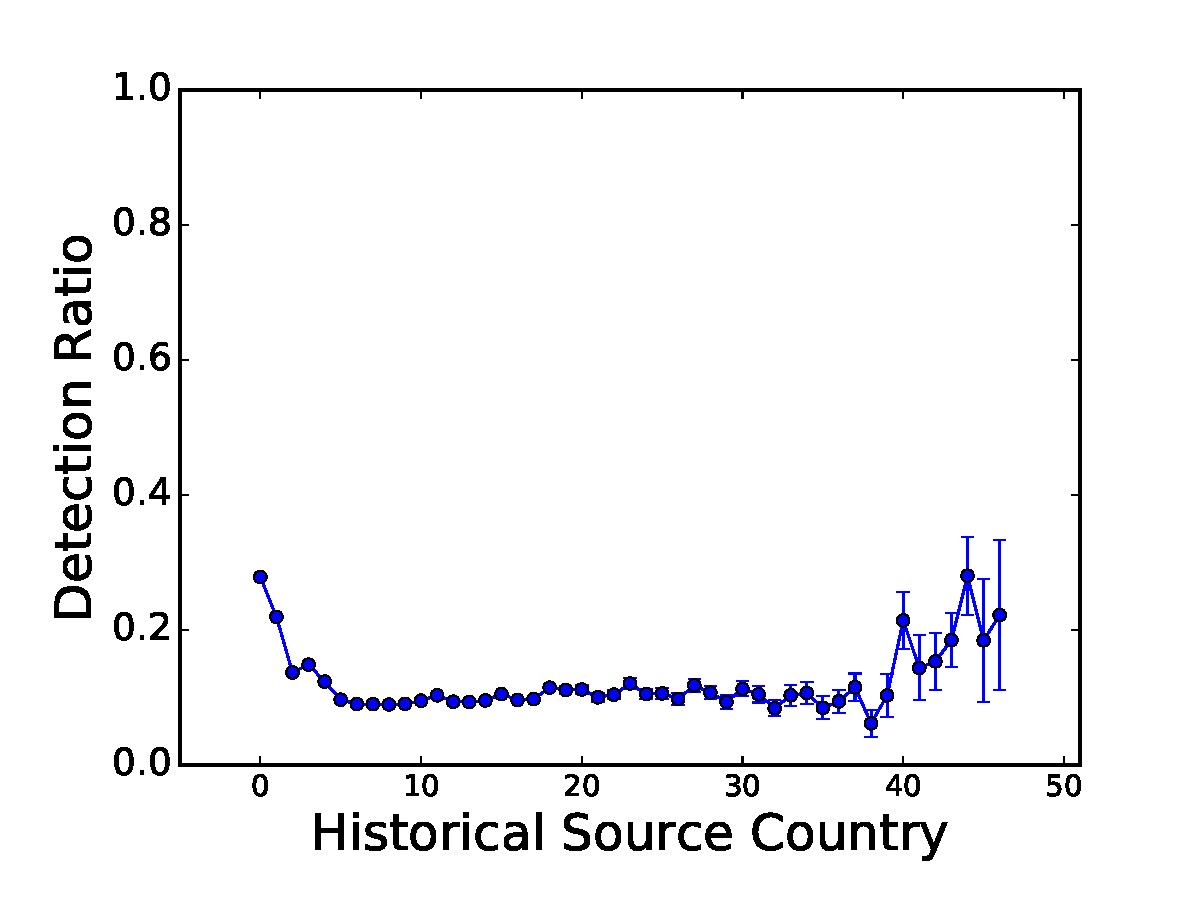
\includegraphics[width=\linewidth]{figure/SubCountry}
  \mycaption{fig:hiscountry}{The relation between the number of historical source countries and detection rate.}
{\footnotesize{(How detection rate changes with the number of historical source countries.
95\% confidence interval is also drawn for each point.)}}
\endminipage\hfill
\minipage{0.31\textwidth}
  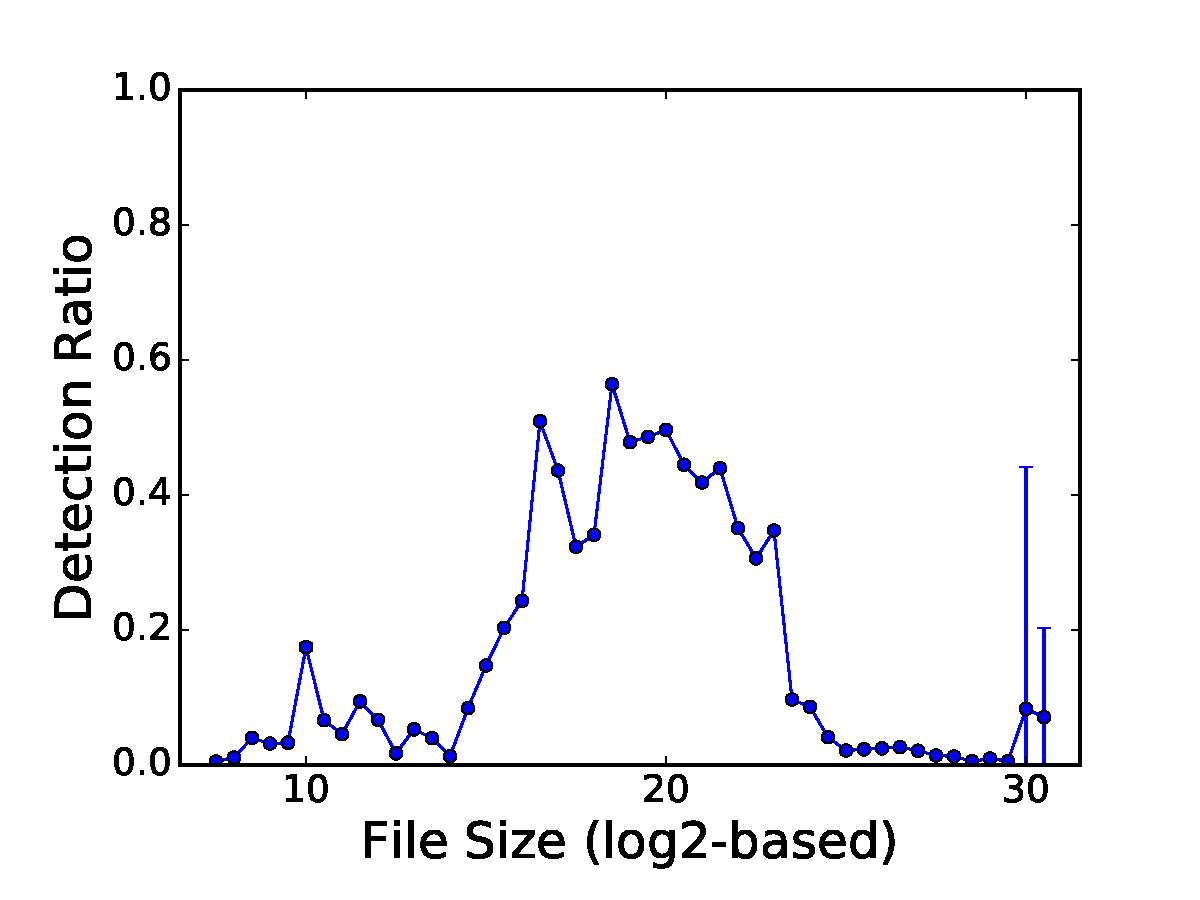
\includegraphics[width=\linewidth]{figure/size}
  \mycaption{fig:size}{How detection rate changes with file size.}
  {\footnotesize{(How detection rate changes with log2-based file size.
Results from log2 are rounded up to nearest 0.5.
95\% confidence interval is also drawn for each point.)}}
\endminipage\hfill
\minipage{0.31\textwidth}%
  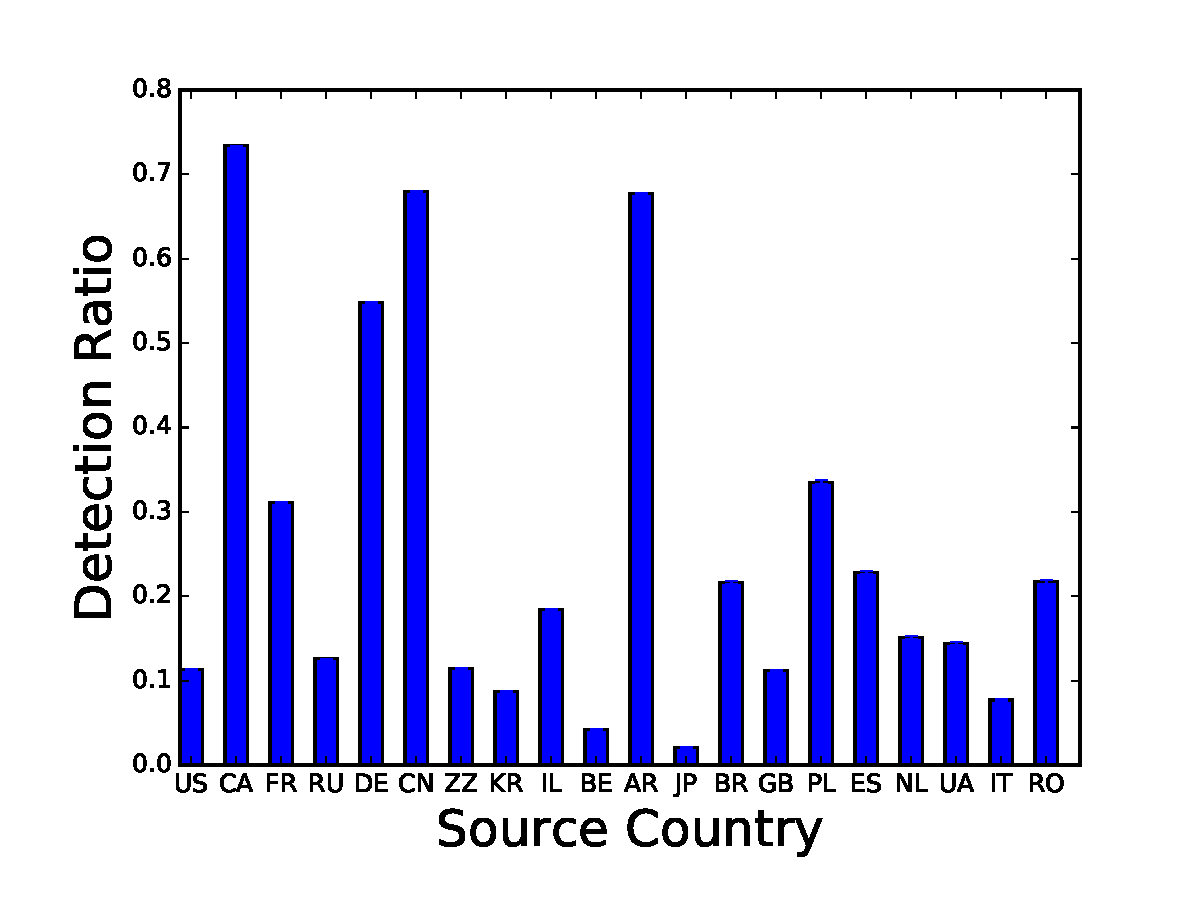
\includegraphics[width=\linewidth]{figure/Country}
  \mycaption{fig:Country}{Average detection rate for top 20 countries.}
{\footnotesize{(Average detection rate for submissions from countries ranking 
in top 20 in making PE submissions to VirusTotal. 
95\% confidence interval is also drawn for each country.)}}
  %\label{fig:aveUncover}
\endminipage\hfill

%\vspace{-0.2in}
\end{figure*}



\begin{figure}[t!]
\begin{center}
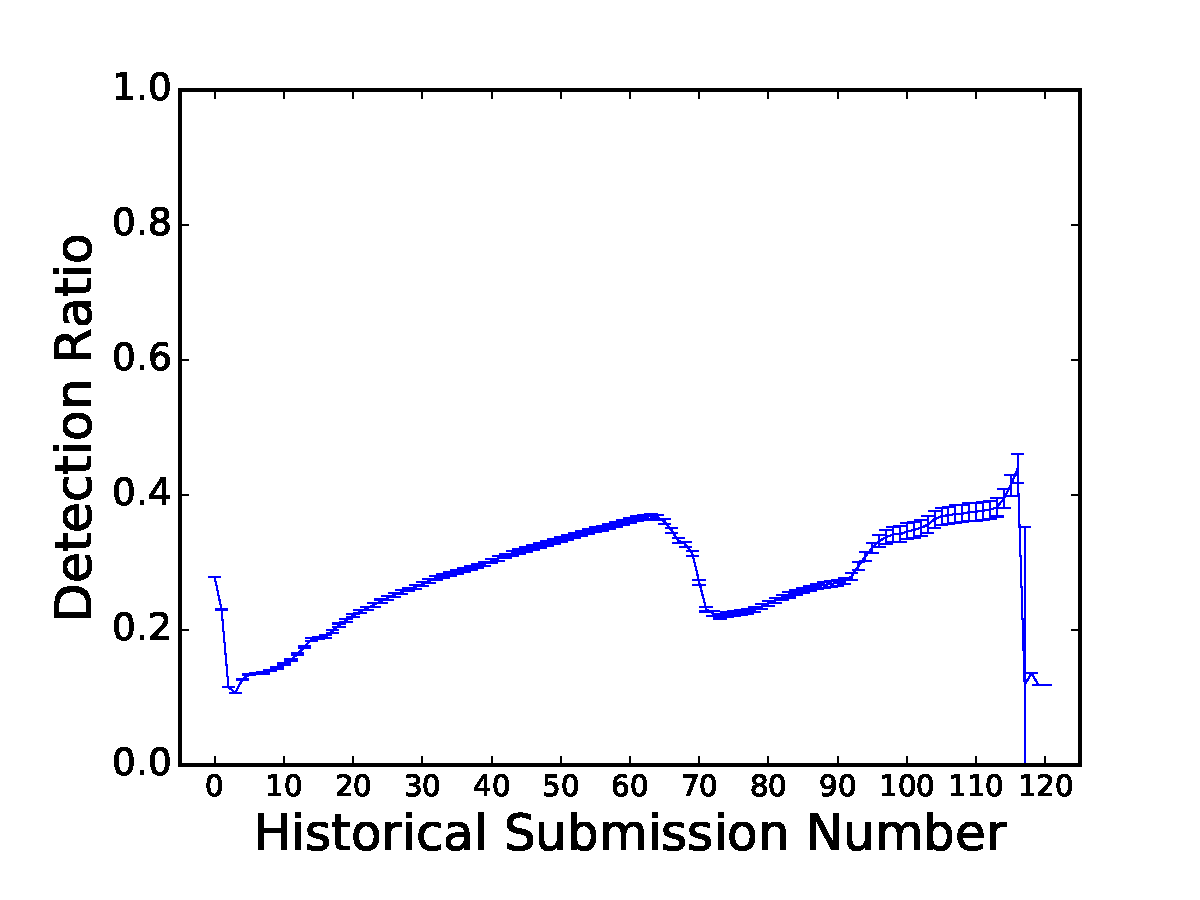
\includegraphics[width=2in]{figure/SubNum}
\caption{
The relation between historical submission number and detection rate.
(
How detection rate changes with historical submission number. 
Each historical submission number is rounded up to nearest 5.
95\% confidence interval is also drawn for each point.
)	
}
\label{fig:hisnum}
\end{center}
%\vspace{-0.25in}
\end{figure}

%\begin{figure}[t!]
%\begin{center}
%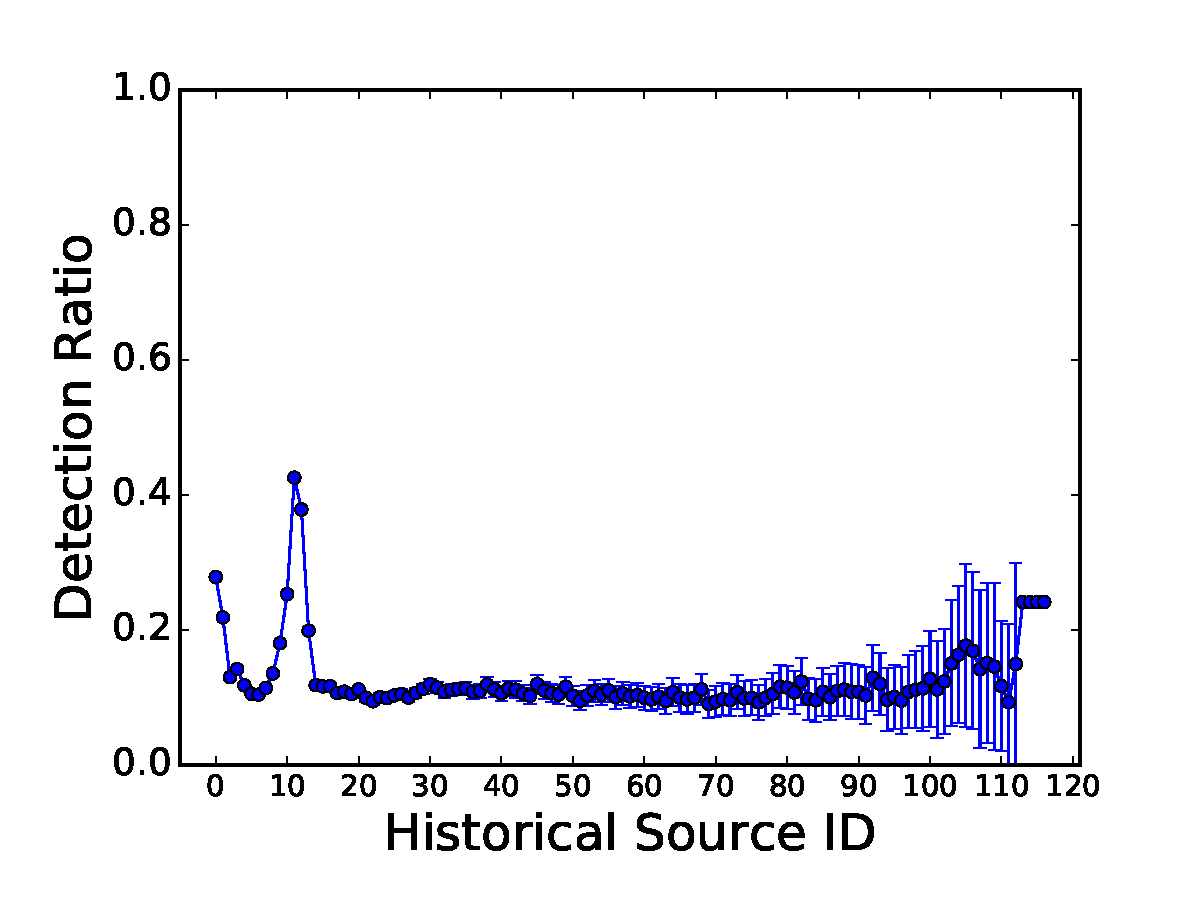
\includegraphics[width=2.5in]{figure/SubID}
%  \mycaption{fig:hisid}{The relation between the number of historical source ids and detection rate.}
%{\footnotesize{(How detection rate changes with the number of historical source ids. 
%Each historical number of source ids is rounded up to nearest 5.
%95\% confidence interval is also drawn for each point.)}}

%\end{center}
%\vspace{-0.25in}
%\end{figure}


As discussed in Section~\ref{sec:basicanal}, there are files that have been submitted more than once to VirusTotal. 
It is worthwhile to investigate this {\em history of submission} and how history affects future.
We study the correlation between submission history and the detection rate of the current submission.
Among the different types of historical information that we study,
we find that two types have higher correlation to detection rate:
the number of submissions made in history and the number of source IDs that made submissions of the same file in history.
%Given a submission, we also study whether information for historical 
%submissions of the same file influences detection rate for the current submission. 

\noindent{\textit{\underline{The number of submissions in history.}}}
To study the submission history, we first sort all submissions for each file chronologically
and then collect the number of all submissions made before submission $s$ for each submission $s$ in \vt.
Next, we calculate the correlation between detection rate and the number of submission in history.
Figure~\ref{fig:hisnum} plots how detection rates change over the number of historical submissions.
Interestingly, there are two main ranges that steadily increase and there are three drops in the beginning, middle, and end.

To explain this effect, we first look at the two factors that can both influence detection rates:
the percentage of benign files submitted and the amount of anti-virus engines labeling the submission as malware.
%Two factors can influence detection rates and explain the above effect.
Obviously, with more benign files submitted, detection rate will decrease.   
and with more engines labeling malwares, detection rate will increase. 
In the the two stages of detection rate increasing, 
with more submissions, more engines are able to identify malwares 
and the increase of percentage of engines identifying submitted malwares dominates. 
In the range that detection rate drops, 
VirusTotal users stop submitting files that have already been identified as malwares,
and the increase of percentage of benign files submitted to VirusTotal dominates. 

\noindent{\textit{\underline{Historical source ID.}}}
One file can be submitted by one source ID multiple times 
and can also be submitted by different source IDs multiple times. 
We now study the correlation between the number of source IDs in the submission history and the detection rate. 

Figure~\ref{fig:hisid} plots the detection rate and confidence interval as the number of historical source IDs increases. 
Confidence intervals are invisible before 80. 
Detection rate is higher for historical source IDs less than 12, compared with historical source IDs more than 12.
\yiying{is it 12? I cannot tell for sure by just looking at the figure}
The number of historical source IDs reflects the popularity of a submitted file.
When the popularity of a file is larger than a certain value, 12 for our dataset, 
file popularity is unrelated to detection rate. 

{\bf Observation 5:} 
{\em }

\if 0
\noindent{\textit{\underline{Historical source country.}}}
One file could also be submitted from different countries. 
The number of historical source countries also reflect the popularity of a submitted file. 
The correlation between detection rate and the number of historical source countries in 
Figure~\ref{fig:hiscountry} shows similar trend as the correlation between detection rate 
and the number of historical source IDs in Figure~\ref{fig:hiscountry}. 

Figure~\ref{fig:hisnum}, Figure~\ref{fig:hisid}, and Figure~\ref{fig:hiscountry} show that 
when historical numbers fall into certain range, they are correlated with detection rate. 
\fi

\subsection{Reputation of Source ID}
\label{sec:reputation}



\begin{figure}[t!]
\begin{center}
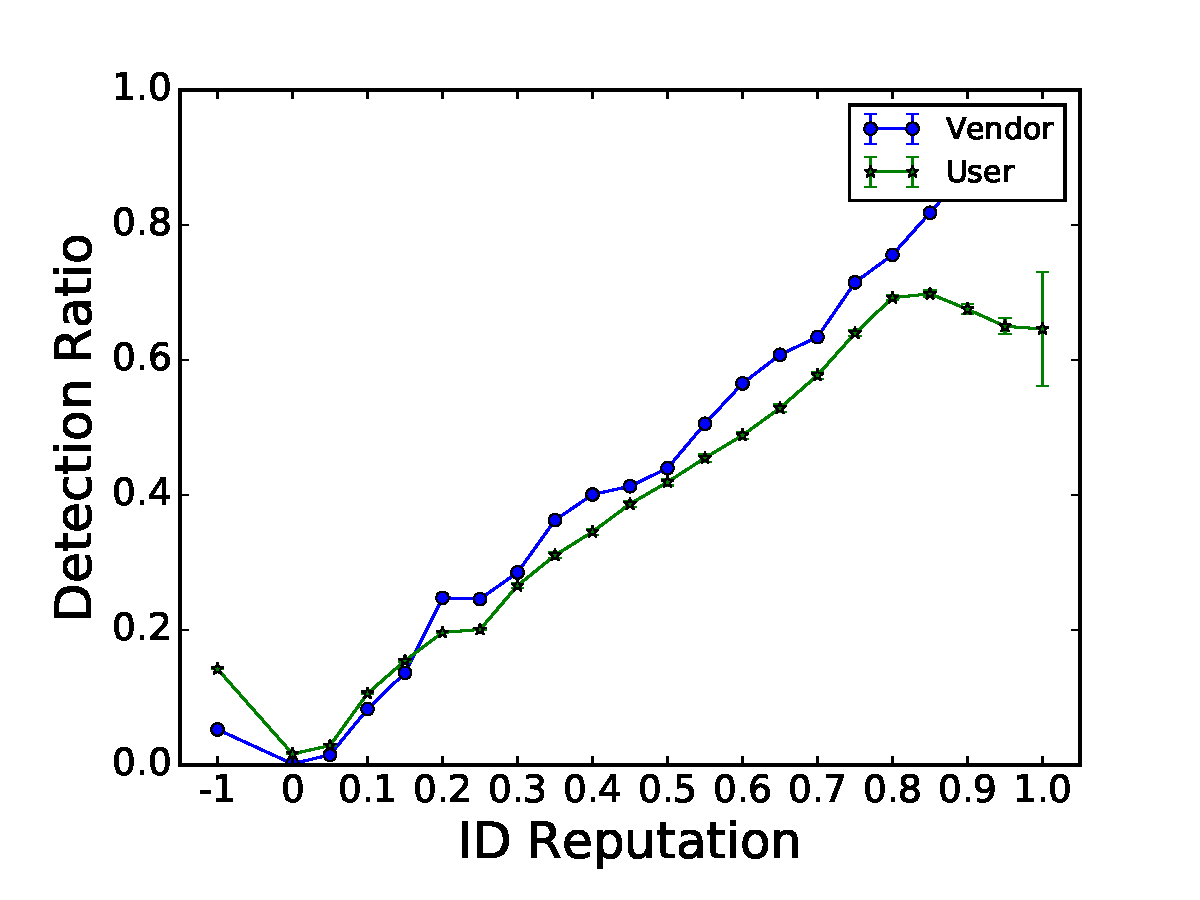
\includegraphics[width=2in]{figure/IDReputation}
\caption{The relation between source id's previous reputation and detection rate.
(How detection rate changes with the value of source id's reputation. 
Each reputation is rounded up to nearest 0.05.
Reputation -1 means the source id did not make any submission before. 
95\% confidence interval is also drawn 
for each point.)
}
\label{fig:idreputation}
\end{center}
%\vspace{-0.25in}
\end{figure}

Previous work~\cite{GuoICSE2010} reported correlation between bug reporter’s reputation and the likelihood for the bug being fixed. 
We also observe correlation between the reputation of source ID and submission’s detection rate. 

%\theoremstyle{definition}
\begin{definition}{Reputation:}
Given a submission $S$ with source ID $N$, 
we define the reputation of $N$ when conducting the submission $S$ as the average detection rate for all submissions conducted by $N$ before $S$. 
If $N$ did not make any submission before, we define the reputation to be $-1$. 
\end{definition}

For around 14\% PE submissions, VirusTotal fails to provide source ID information. 
We filter out these submissions, when computing reputation.
All other PE submissions are conducted by 613 thousand source IDs. 
66\% source IDs only conduct submission once. 
XXX
We filter source IDs conducting more than 1 million PE submissions in our data set, 
because we think these are anti-virus vendors routinely test their products. 

When calculating reputation, we sort all submissions from the same source ID chronologically, 
and calculate reputation for each source id when conducting each submission. 
We round up each calculated reputation to nearest 0.05. 
We group submissions based on source ids' reputation when conducting submissions, 
and we plot average detection rate and 95\% confidence interval for each group in Figure~\ref{fig:idreputation}. 
Except the point with reputation 1, all other confidence intervals are invisible.  

As shown in Figure~\ref{fig:idreputation}, 
there is a rough increase for detection rate as the increase of source ID's reputation, 
with the exception for the point with reputation -1 and the point with reputation 1. 
It is interesting to observe that first submissions conducted by different source IDs have higher 
detection rate than submissions conducted by IDs with reputation 0, 
and it is difficult for source IDs with highest reputation to always submit files detected by all engines. 
Correlation between source ID's reputation and detection rate indicates 
that it is feasible to use source IDs' submission history to predict their future submissions.

{\bf Observation 6:} 
{\em }

\subsection{Discussion}

\noindent{\textit{\underline{How to use our data?}}}
File size, historical number in certain range, and source ID reputation
are highly correlated with detection rate. 

A possible future work could train a regression model to combine all these factors together and 
predict how many engines could detect a malware or how likely a file is a malware. 
Using the regression model or our studying results alone, 
security experts can prioritize malwares and focus their efforts on malwares which are more malicious. 
Anti-virus vendors could inspect results which are variant from our studying results 
to identify possible false positives or false negatives in their products. 

\yiying{I would delete the following paragraph. it just sounds too defensive. and you've already explained the limitation in sec 2.4.}
\noindent{\textit{\underline{Limitations of our study.}}}
As discussed in Section~\ref{sec:meth}, our study is bound with our methodology.
We do not have any data before 05/07/2016, 
which may cause some inaccuracy in measuring historical statistics and 
source ID reputation and historical numbers.
However, we think we can tolerate this error, 
since we conduct our study in a relatively long time range and in a large scale. 
%In the future, we could design our reputation and historical metrics based on a tunable time windows, and investigate whether correlations still exist.   
